\chapter{METHODOLOGY}
\section{Overview}

The methodology for the stock market tracking, prediction, and notification system follows a structured approach, starting with a thorough requirement analysis to define key features such as stock tracking, goal setting, and real-time alerts. The system is designed to ensure modularity, scalability, and independent development, where each service handles specific tasks like data fetching, machine learning predictions, goal matching, and user management. Data are collected from APIs of the stock market, pre-processed, and used to train machine learning models for trend prediction. The backend processes user input, compares predictions with goals, and triggers notifications via WebSockets or push notifications. The front-end is developed with React for real-time data visualization and user interactions.  Finally, the performance of the system is monitored, and periodic retraining of the model ensures the accuracy of the predictions.
\section{Frontend (User Interface)}

\subsection{React}
React is a popular JavaScript library for building user interfaces, particularly for single-page applications. Developed by Facebook, it allows developers to create reusable UI components that efficiently update and render data as the application state changes. React uses a virtual DOM to optimize performance, ensuring faster updates and a smooth user experience. It is widely used for building dynamic web and mobile apps due to its simplicity, flexibility, and scalability.

\subsection{Ui Library}Material-UI or Tailwind CSS are utility-first CSS frameworks that allows developers to design custom user interfaces by applying utility classes directly in HTML. It promotes a highly flexible and component-based approach, enabling rapid styling and easier customization without writing custom CSS

\subsection{Redux }
Manage global state for user settings, goal prices, and real-time stock updates.Redux is a state management library for JavaScript applications, commonly used with React. It provides a centralized store to manage application state, ensuring predictable and consistent behavior. Redux uses actions and reducers to handle state updates, making it easier to debug, test, and manage complex state changes across large applications
\section{Backend (API and Core Logic)}
The backend handles user requests, processes data, and delivers responses. It’s the heart of the system.
\subsection{Node.js with Express.js:}
\begin{itemize}


    \item Lightweight and efficient for REST API development.
    \item Routes handle operations like fetching stock data, updating user settings, and delivering predictions
\end{itemize}
\subsection{Database}
\begin{itemize}
    \item PostgreSQL
    \begin{enumerate}
        \item PostgreSQL excels at managing structured data where relationships between entities (e.g., users and their stock goals) are critical.
        \item Serve as the primary database for backend services that handle user authentication, goal management, and preferences.
    \end{enumerate}
    \item MongoDB 
    \begin{enumerate}
        \item Stock market data, such as price movements, trading volume, and historical records, are typically time-stamped.
        \item Stock data can vary depending on the API or data source. MongoDB's schema-less design accommodates changes in data structure without requiring schema migrations.
        \item MongoDB supports horizontal scaling, which is essential for handling large volumes of real-time stock market data from multiple sources.
    \end{enumerate}
    \item External APIs \\{APIs to handle :}
  \begin{enumerate}
  
      \item User authentication.
      \item Stock Data retrieval
      \item Goal setting and alerts
  \end{enumerate}
    
\end{itemize}

\subsection{Algorithm and  Data processing}
This module is crucial for predictive analysis and identifying trends.
\begin{enumerate}
    \item \textbf{Python for Data Processing}
    \begin{itemize}
        \item \textbf{Pandas}: Cleaning and structuring historical stock data.
        \item \textbf{NumPy}: Efficient numerical calculations.
        \item \textbf{Matplotlib/Seaborn}: Data Visualization during development and debugging
        \item \textbf{Tensorflow}: 
TensorFlow stock price prediction involves using machine learning models to analyze historical market data and forecast future stock prices. It leverages neural networks and deep learning techniques for accurate predictions. This approach aids in making data-driven investment decisions.
    \end{itemize}
    \item \textbf{Machine Learning}
    \begin{itemize}
        \item \textbf{Supervised Learning Models}
        \begin{itemize}
            \item \textbf{Linear Regression} for simple trend predictions.
            \item \textbf{Long Short-Term Memory} 
            \begin{itemize}
                \item \textbf{Captures Temporal Patterns}: Recognizes sequential dependencies in stock price movements.
                \item \textbf{Predicts Future Prices}: Forecasts trends and price movements based on historical data.
                \item \textbf{Detects Patterns and Anomalies}: Identifies trend reversals and irregular market activity
                \item \textbf{Processes Multi-Feature Data}: Integrates prices, volumes, and indicators for richer insights.
                \item \textbf{Solves Vanishing Gradient}: Efficiently learns from extended sequences via gating mechanism.
            \end{itemize}
        \end{itemize}
    \end{itemize}
\end{enumerate}

\section{System Design}
\begin{description}
    \item[Data Flow Diagram (DFD)] is a visual representation of how data moves through a system, illustrating the flow of information between processes, data stores, and external entities. It provides a clear overview of the system's data processing, highlighting how inputs are transformed into outputs. DFDs are typically divided into multiple levels, with higher-level diagrams offering a broad overview and lower-level diagrams detailing specific processes. They are commonly used in system design and analysis to ensure efficient data handling and to identify potential bottlenecks or inefficiencies in the system.
    \item [A sequence diagram]A sequence diagram is a type of interaction diagram because it describes how—and in what order—a group of objects works together. These diagrams are used by software developers and business professionals to understand requirements for a new system or to document an existing process.
\end{description}
\begin{figure}[h]
    \centering
    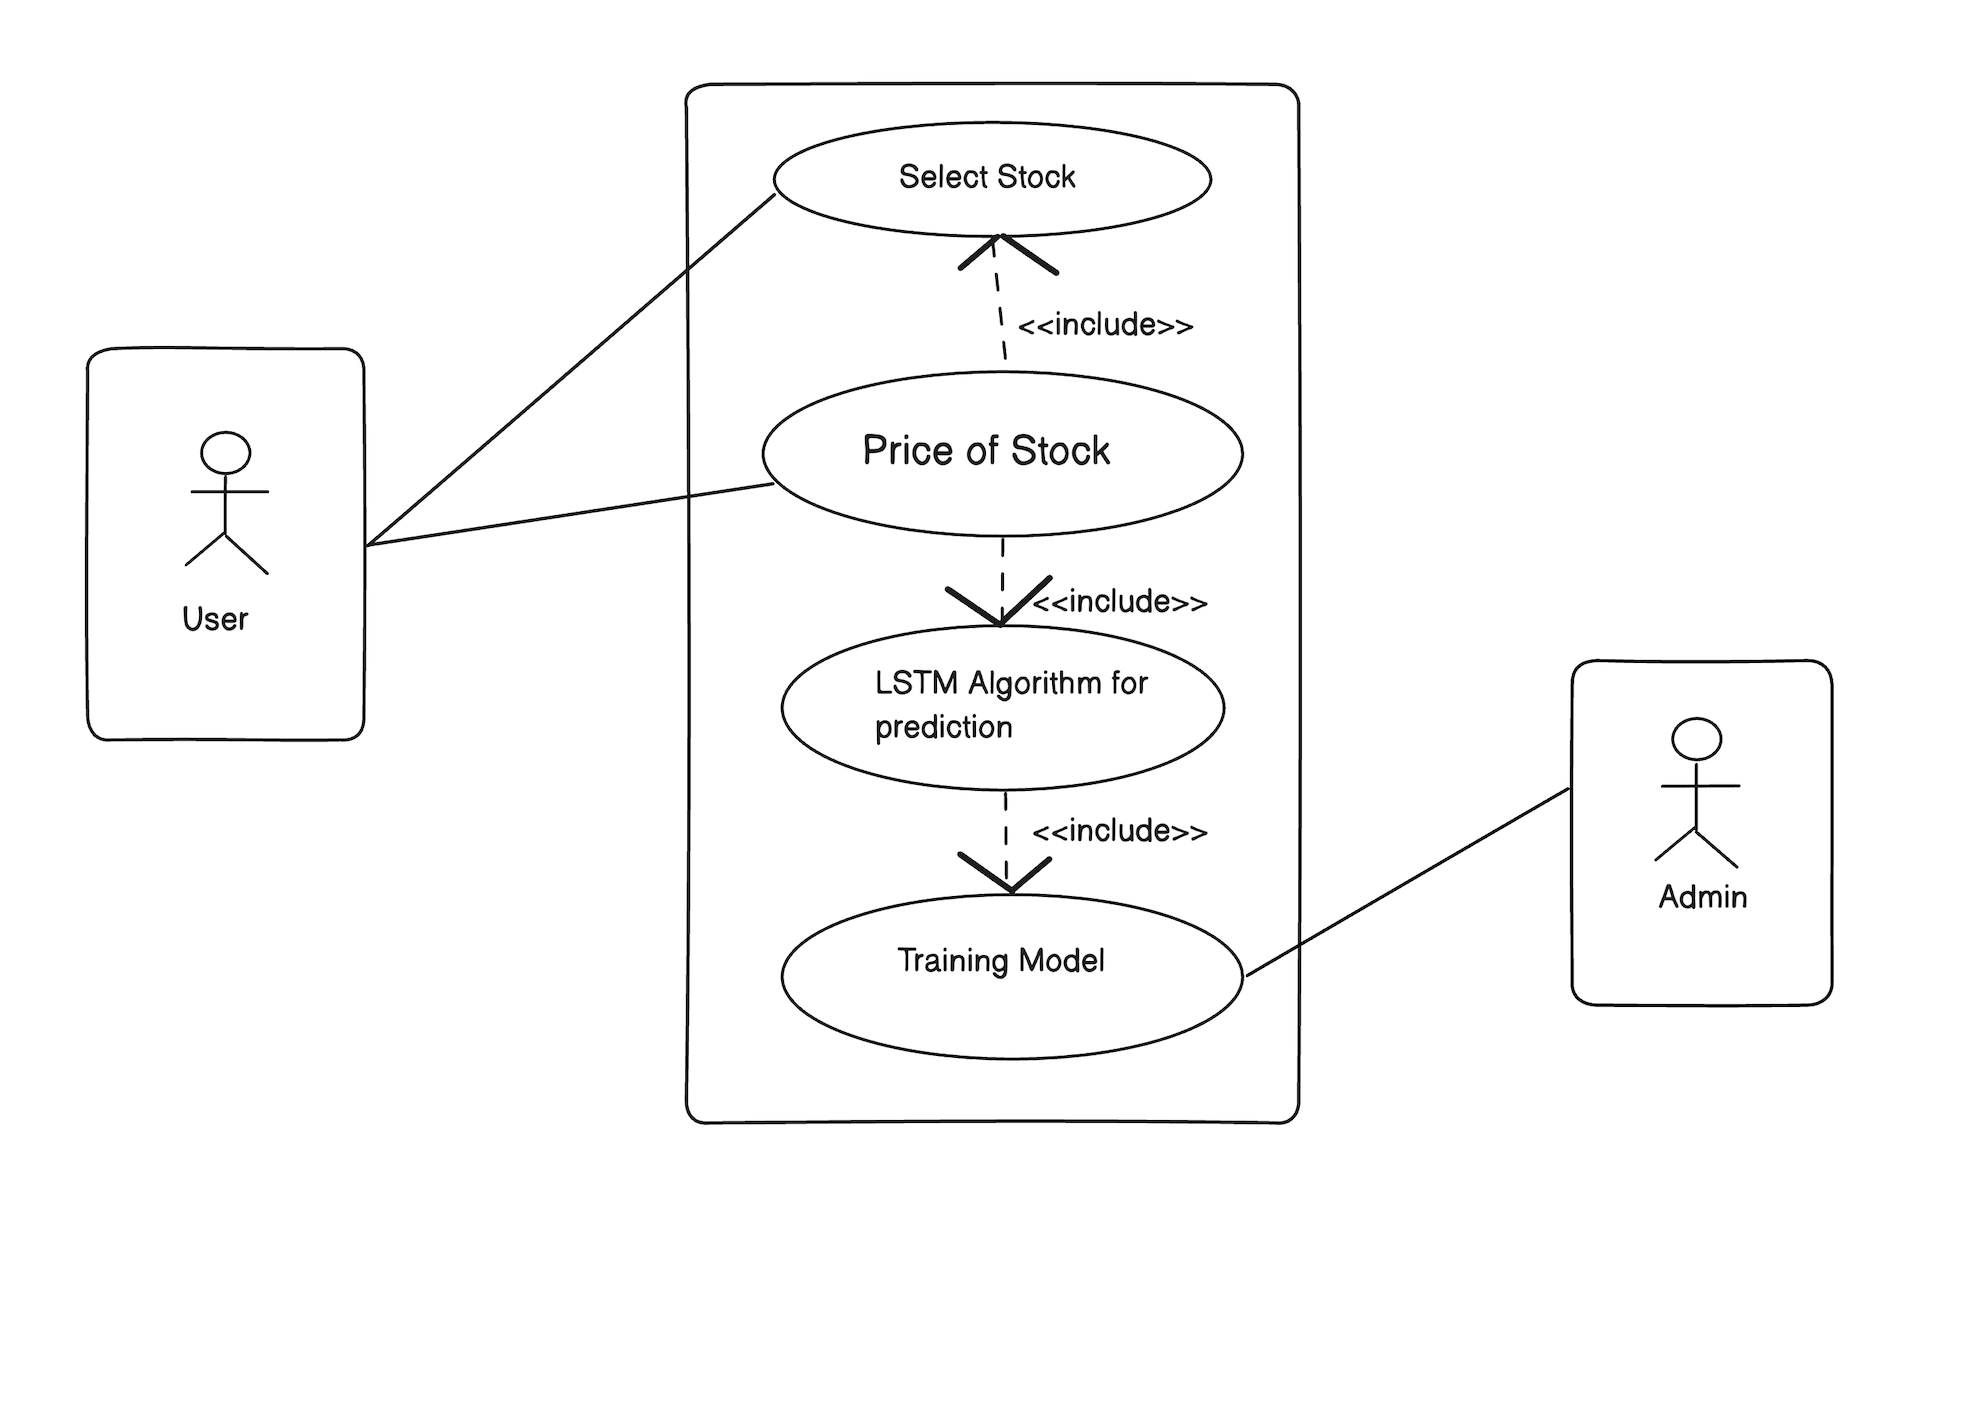
\includegraphics[width=1\textwidth]{Graphics/use_case.png}  
    \caption{Use Case Diagram}
    \label{fig:example}  
\end{figure}
\begin{figure}[h]
    \centering
    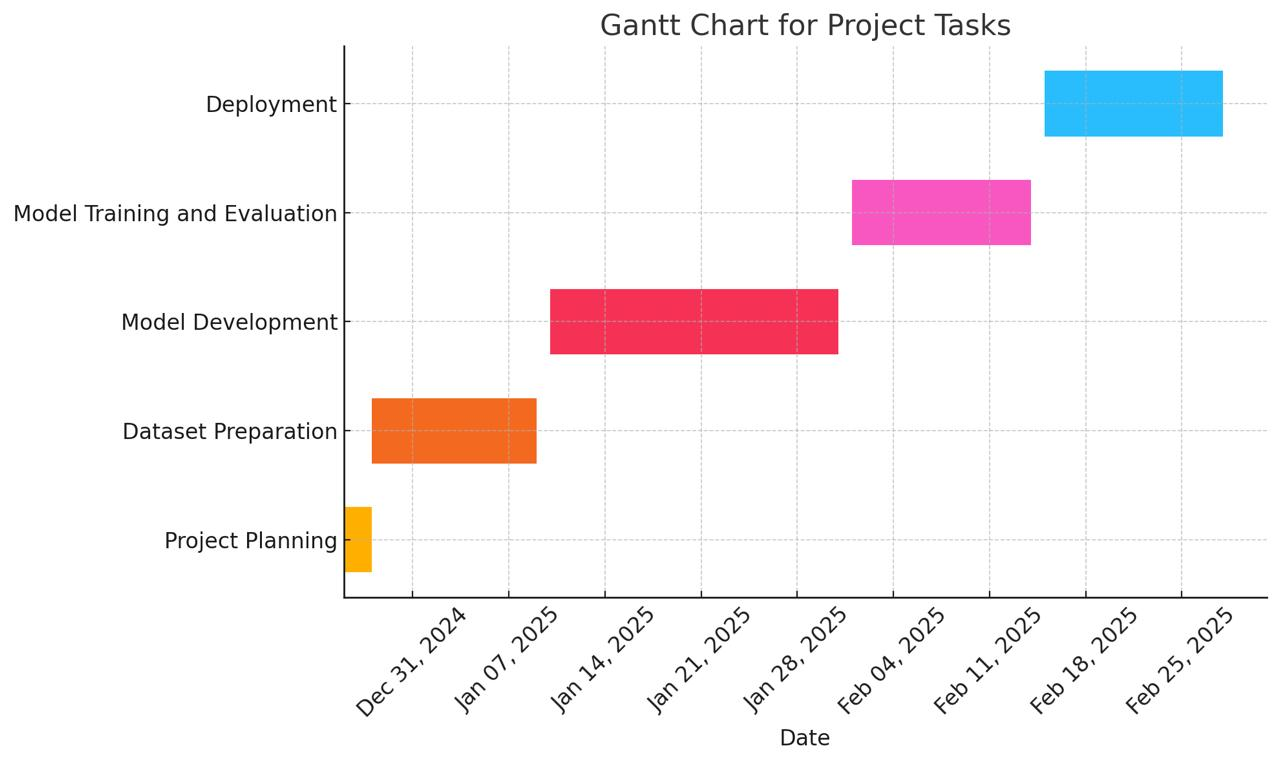
\includegraphics[width=1\textwidth]{Graphics/gantt.jpeg}  
    \caption{Gantt Chart}
    \label{fig:example}  
\end{figure}
\begin{figure}[h]
    \centering
    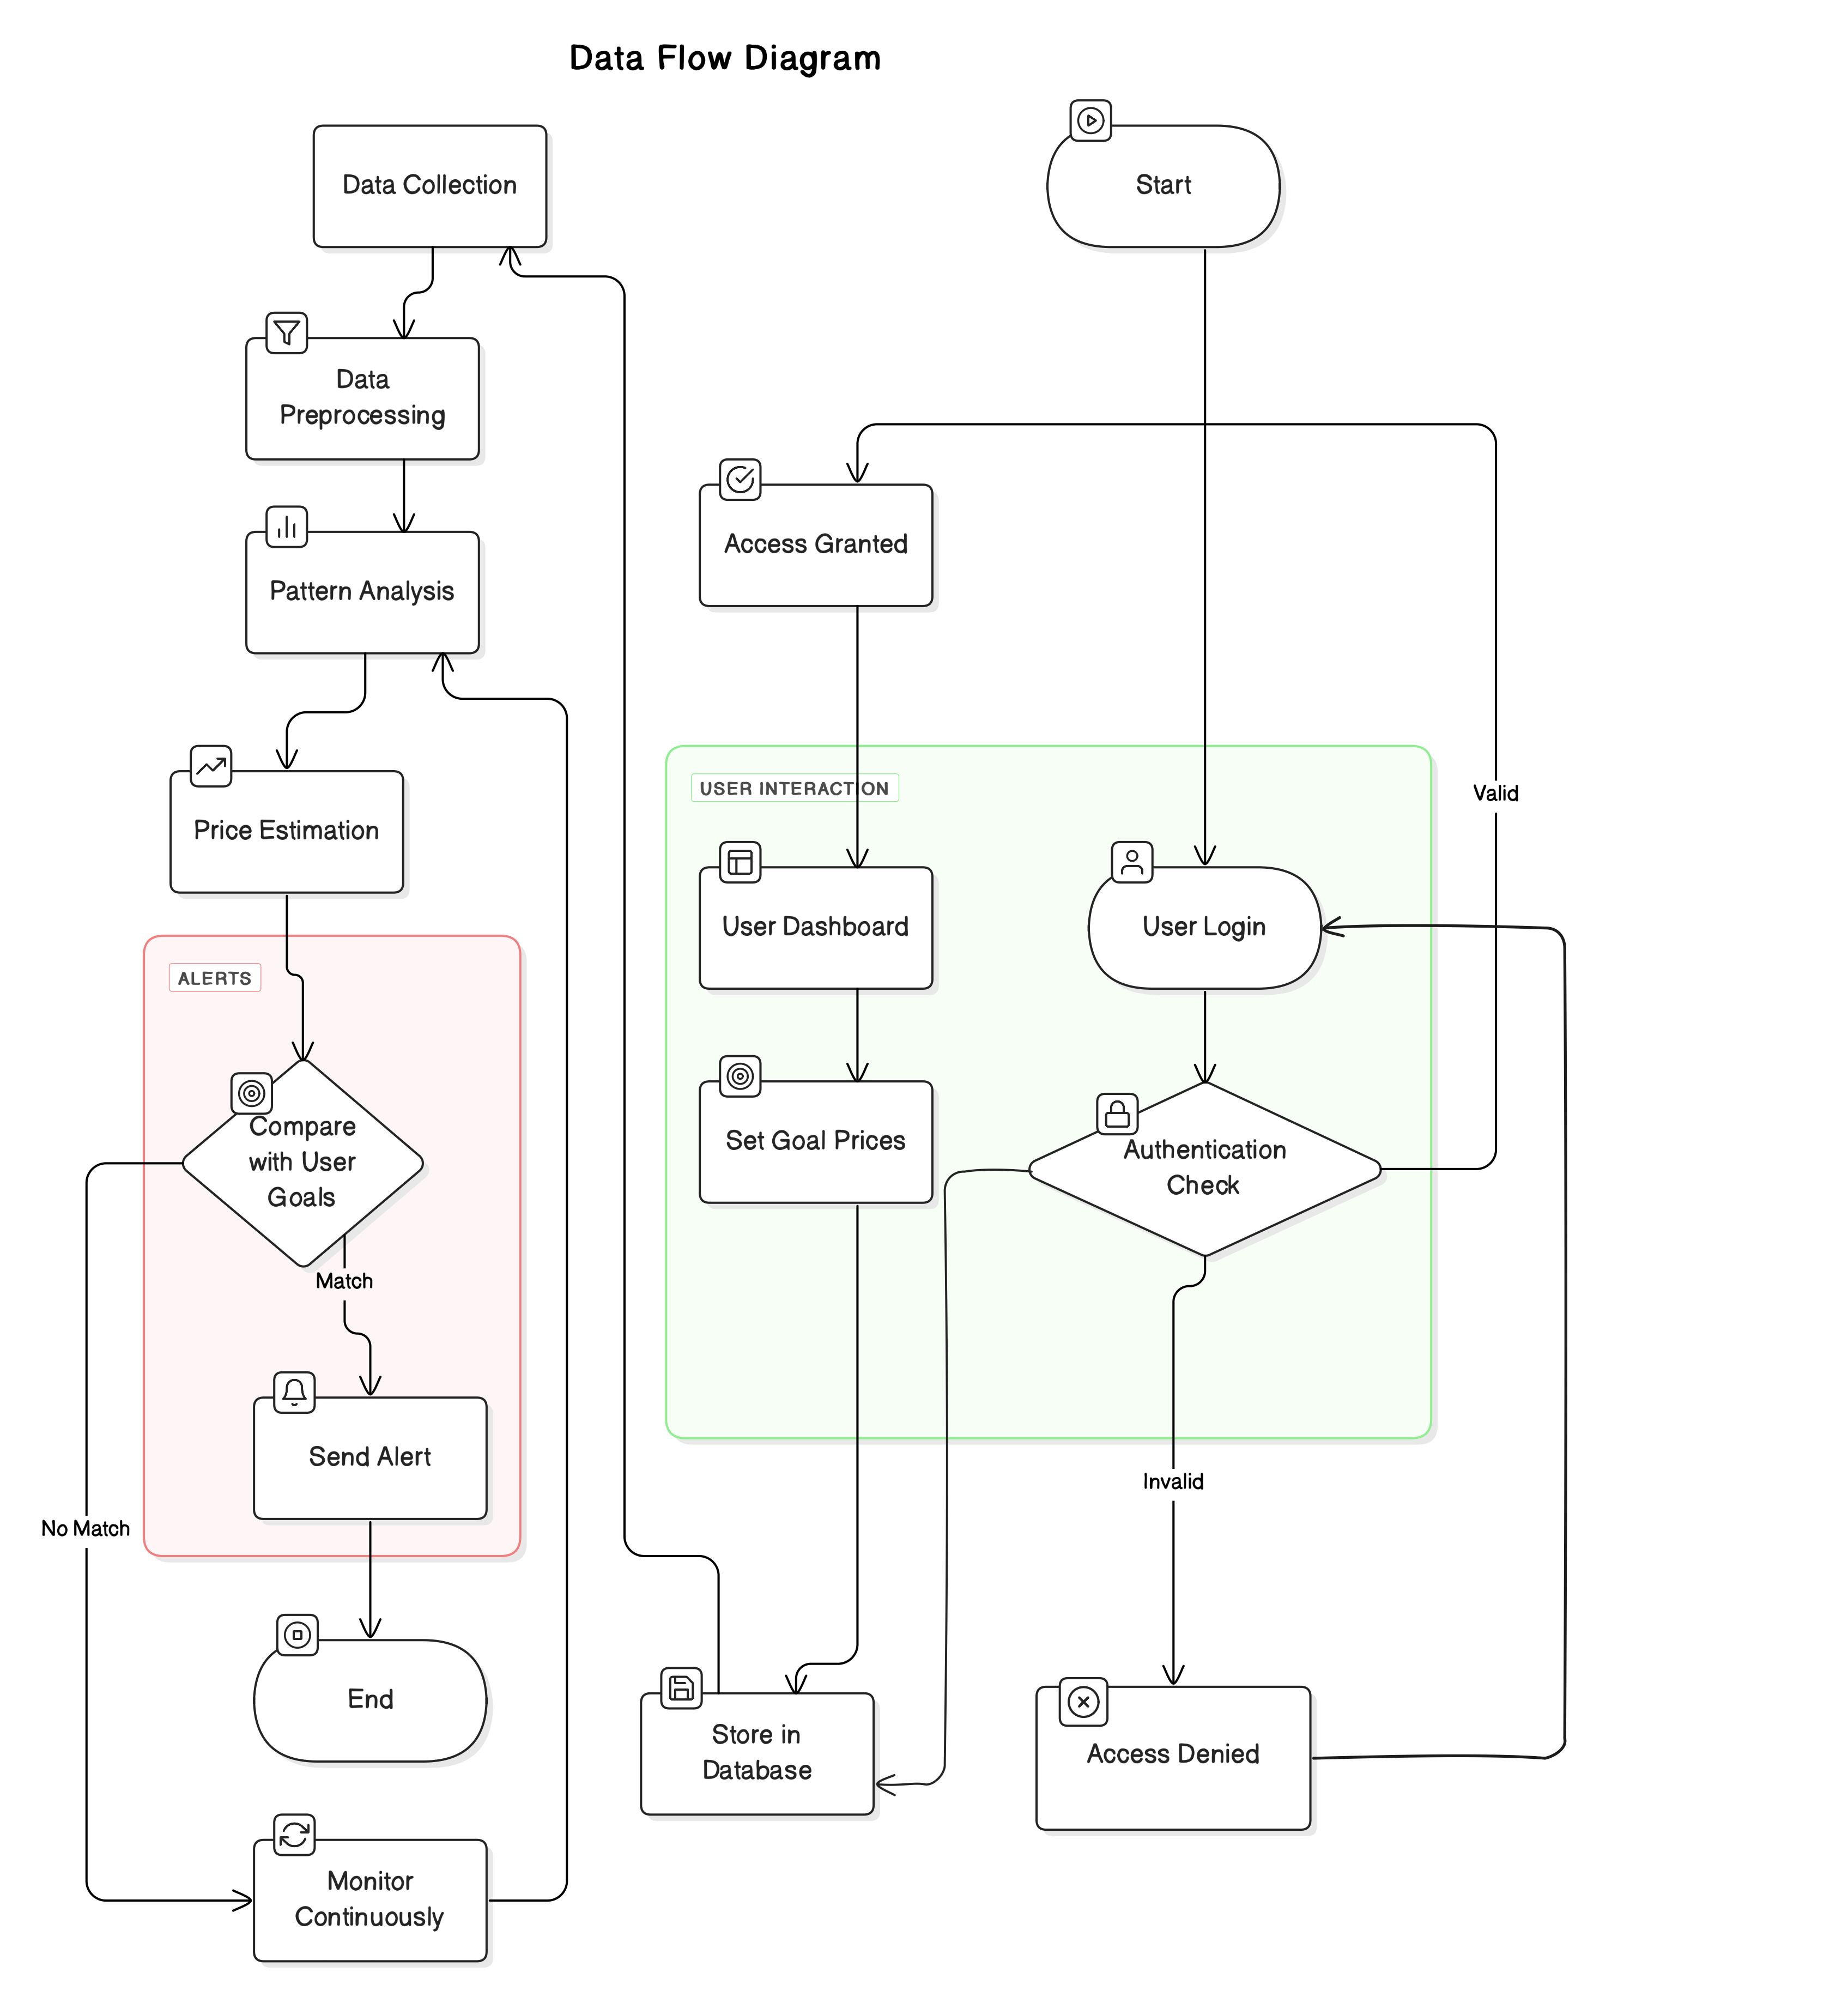
\includegraphics[width=1.2\textwidth]{Graphics/data_flow.png}  
    \caption{Data Flow Diagram}
    \label{fig:example}  
\end{figure}
\begin{figure}
    \centering
    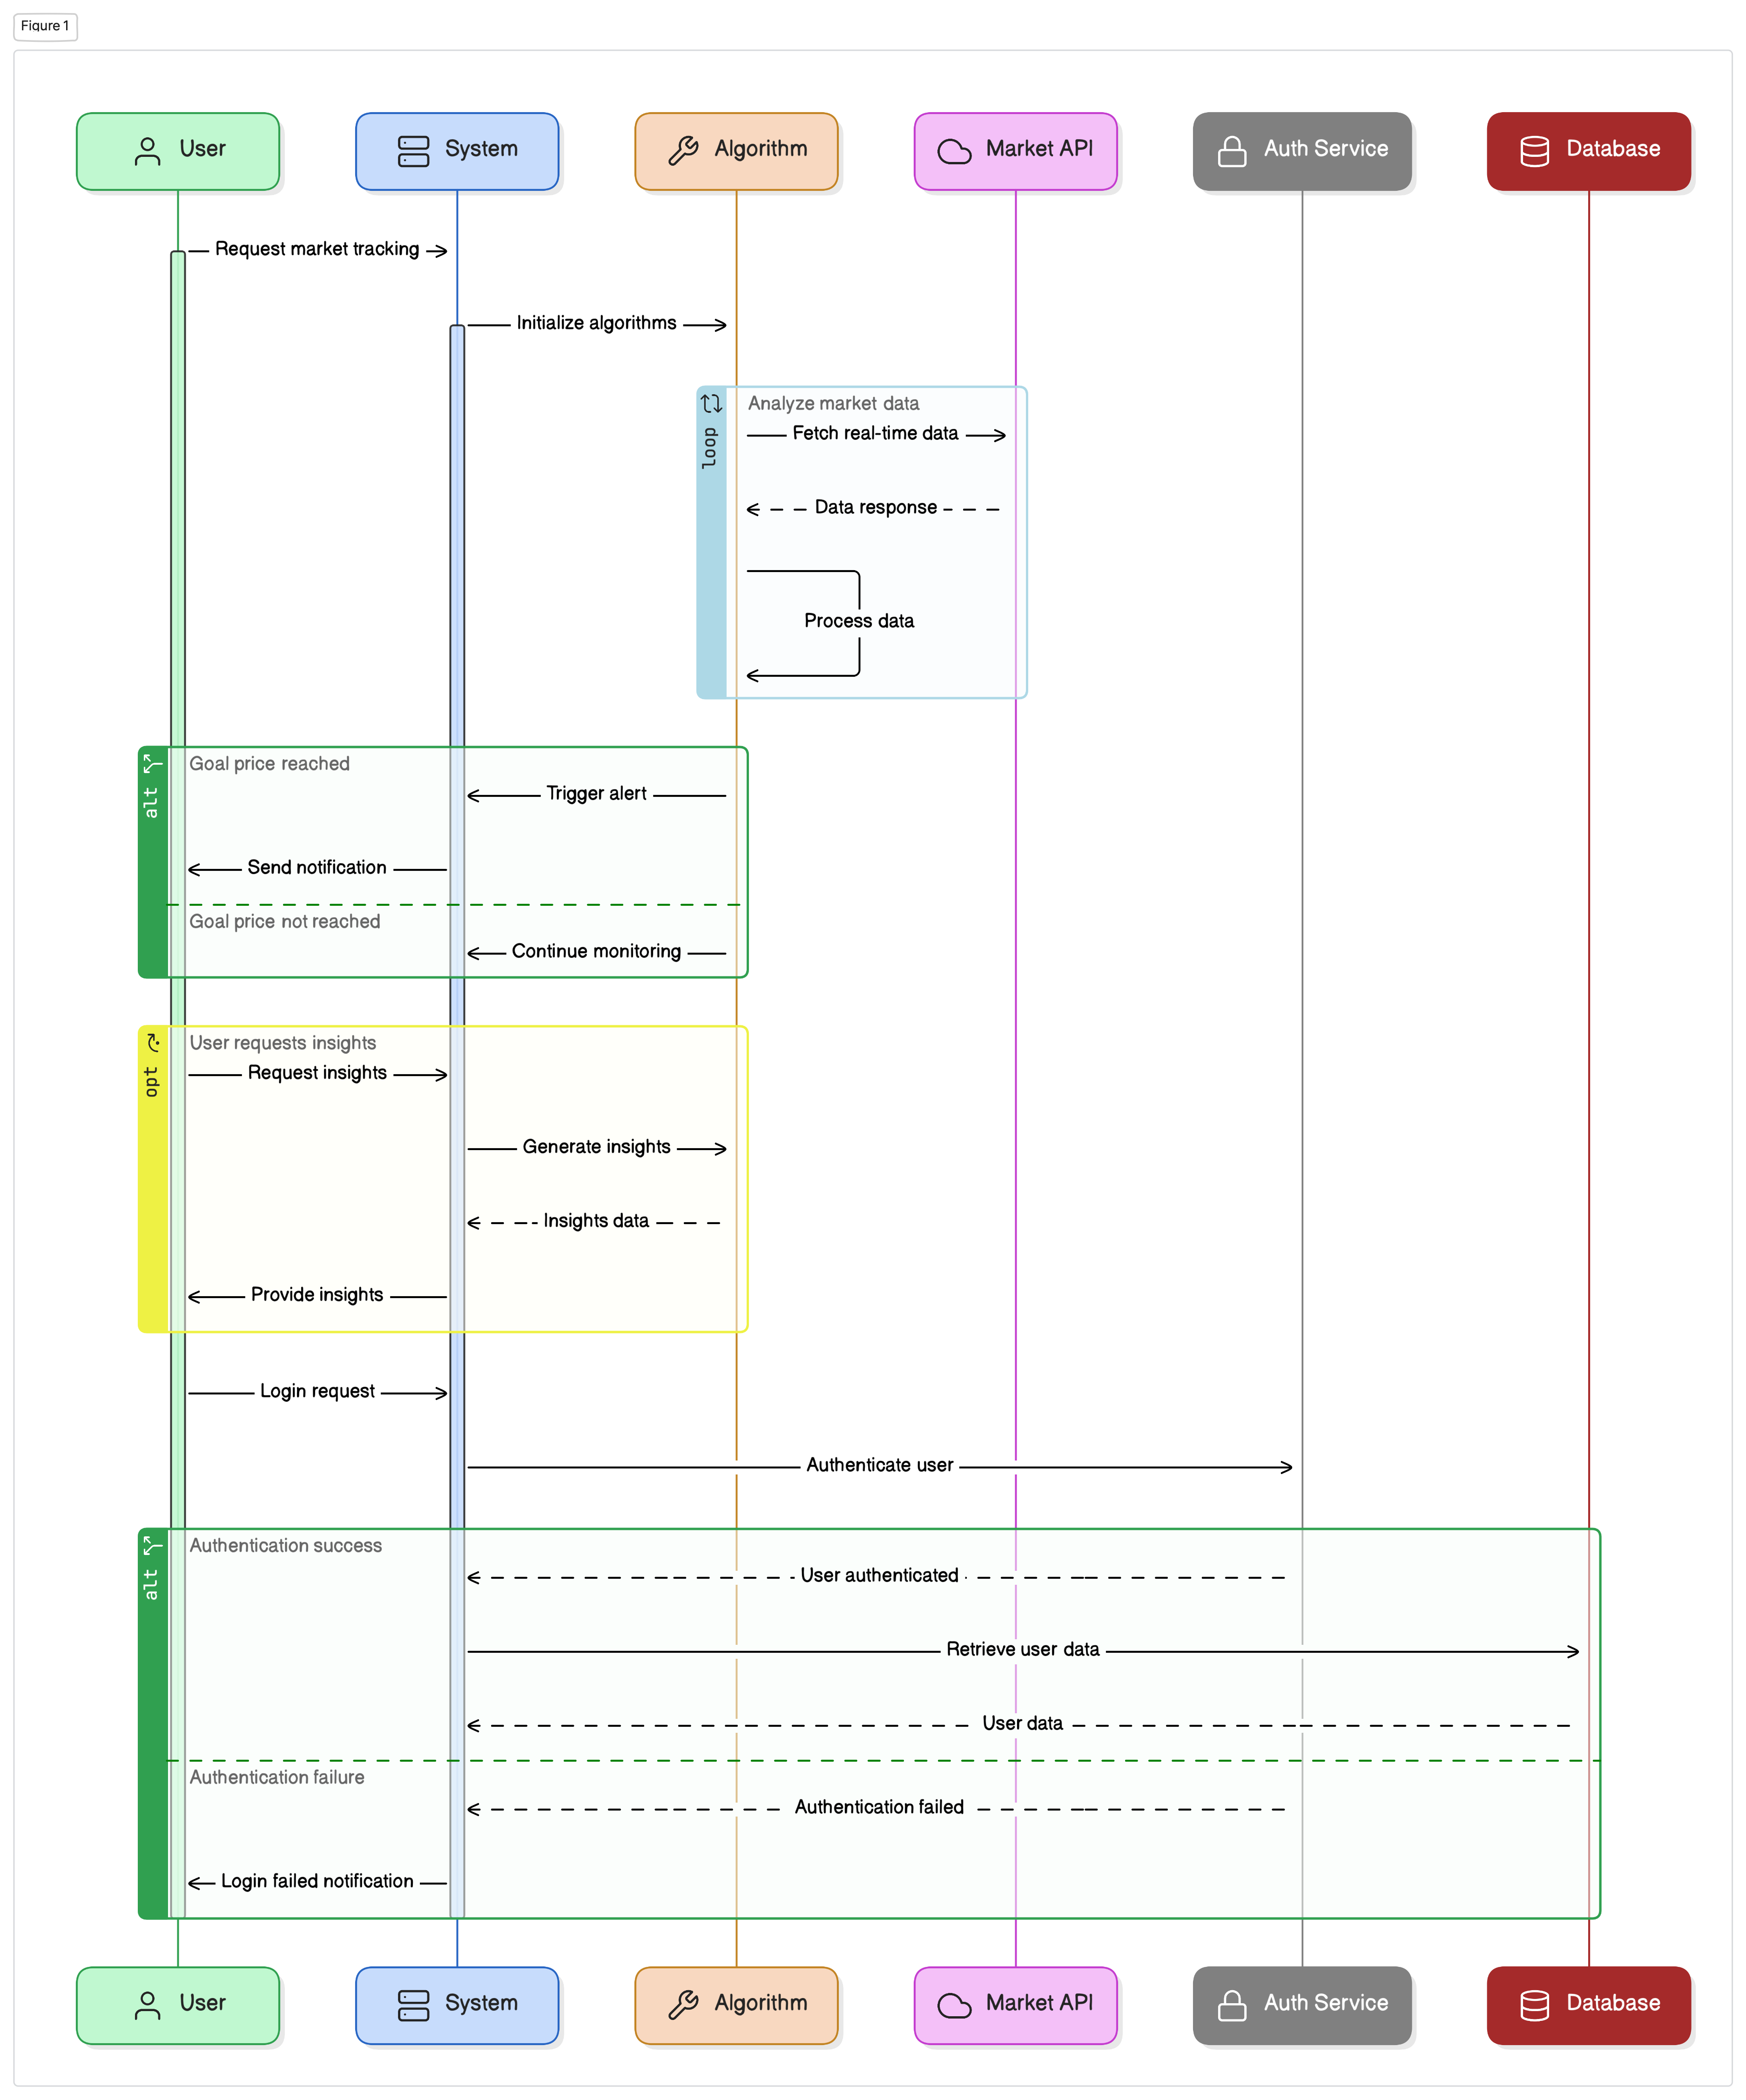
\includegraphics[width=1.1\textwidth]{Graphics/sequence.png}
    \caption{Sequence Diagram}
    \label{fig:enter-label}
\end{figure}
   % \centering
    
   %  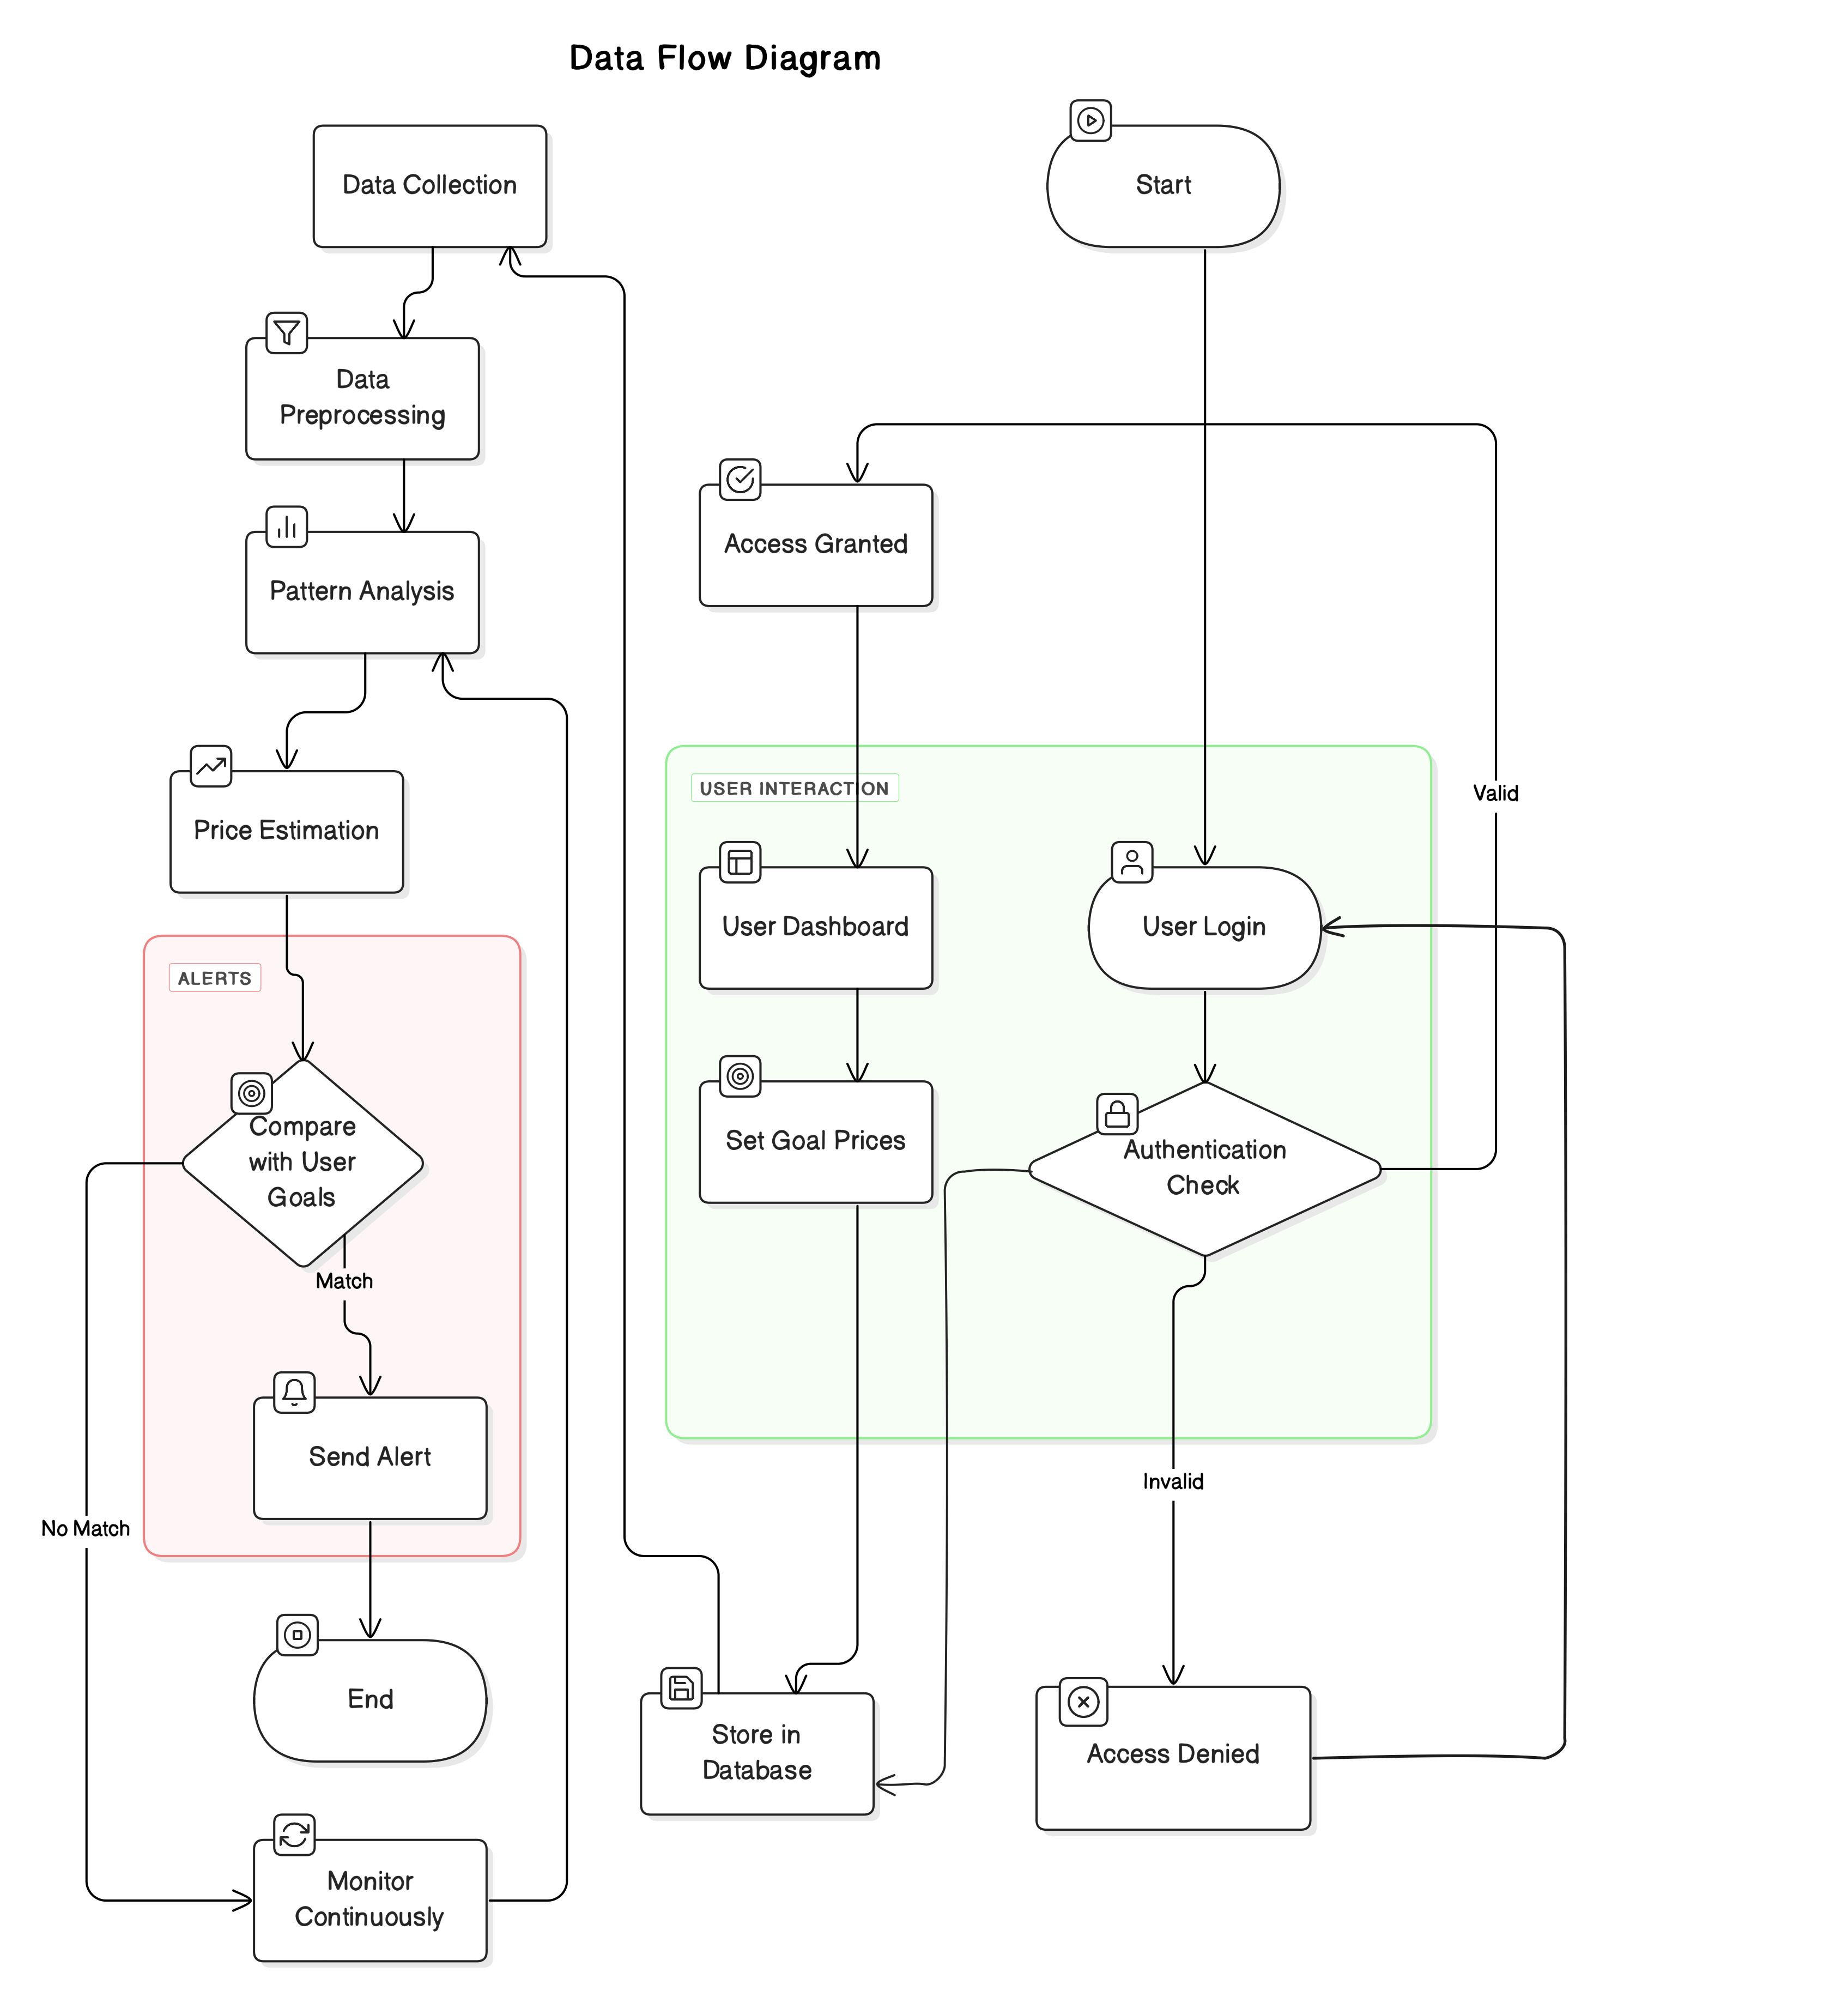
\includegraphics[width=1\textwidth]{Graphics/data_flow.png}\par
   %  \vspace{1.cm}

